% \documentclass{article}
\documentclass[accepted]{uai2023}
\usepackage[american]{babel}

\usepackage[utf8]{inputenc}
\usepackage{csquotes}

\usepackage{amsmath}
\allowdisplaybreaks
\usepackage{mathtools}
\usepackage{bm}
% \usepackage[a4paper, total={7in, 9in}]{geometry}
\usepackage{amssymb}
\usepackage{listings}
\usepackage{soul}
% \usepackage[sorting=none]{biblatex}
%     \addbibresource{references.bib}
\usepackage{natbib} % has a nice set of citation styles and commands
    \bibliographystyle{plainnat}
    \renewcommand{\bibsection}{\subsubsection*{References}}

\usepackage{hyperref}
\usepackage{algorithm}
\usepackage{algpseudocode}
\usepackage{subfig}


\newcommand{\vect}[1]{\mathbf{#1}}
% \newcommand{\eq}[1]{Eq. \ref{#1}}
\newcommand{\px}[1]{\cfrac{\partial #1}{\partial x}}
\newcommand{\py}[1]{\cfrac{\partial #1}{\partial y}}
\newcommand{\dx}[1]{\cfrac{\mathrm{d} #1}{\mathrm{d} x}}
\newcommand{\dy}[1]{\cfrac{\mathrm{d} #1}{\mathrm{d} y}}
\newcommand{\dt}[1]{\cfrac{\mathrm{d} #1}{\mathrm{d} t}}
\newcommand{\ds}[1]{\cfrac{\mathrm{d} #1}{\mathrm{d} s}}
\newcommand{\dnt}[2]{\cfrac{\mathrm{d}^{#1} #2}{\mathrm{d} t^{#1}}}
% \newcommand{\Err}{\mathcal{E}}
\newcommand{\Err}{\eta}
\newcommand{\Bound}{\mathcal{B}}
\newcommand{\Loss}{\mathrm{Loss}}
\newcommand{\Net}{\mathrm{Net}}
\renewcommand{\L}{\mathcal{L}}
\newcommand{\I}{\mathcal{I}}
\newcommand{\Int}[1]{e^{#1 t} \int_{0}^{t} e^{- #1 \tau}\mathrm{d}\tau}
\newcommand{\Intt}{\int_{0}^{t}\mathrm{d}\tau}
\renewcommand{\Re}[1]{\mathcal{R}e\left(#1\right)}
\newcommand{\abs}{|\cdot|}


\title{Residual-Based Error Bound for Physics-Informed Neural Networks}
% \author{Shuheng Liu, Xiyue Huang, Pavlos Protopapas}
% \date{\today}
\setlength{\parindent}{0pt}
% \setlength{\parskip}{1em}

\author[1]{Shuheng Liu}
\author[2]{Xiyue Huang}
\author[3]{Pavlos Protopapas}
% Add affiliations after the authors
\affil[1, 3]{
    Institute for Applied Computational Science\\
    Harvard University\\
    Cambridge, Massachusetts, USA
}
\affil[2]{
    Data Science Institute\\
    Columbia University\\
    New York, New York, USA
}

\begin{document}
\maketitle

\begin{abstract}
    Neural networks are universal approximators and are studied for their use in solving differential equations.
    However, a major criticism lies in that there lacks estimation of error bounds for the obtained solutions.
    This paper proposes a technique to rigorously evaluate the error bound of Physics-Informed Neural Networks (PINNs) on common classes of ODEs and PDEs.
    The error bound is based purely on equation structure and equation residuals, and does not depend on assumptions of how well the networks are trained.
    The technique evaluates the error bound in an efficient manner, and can be further improved to provide tighter bounds at the cost of longer run time.
\end{abstract}

\section{Introduction}
    Differential equations (DEs) are a useful mathematical tool in describing various phenomena in natural sciences, engineering, and humanity studies. 
    As universal approximators, neural networks proves to be powerful in approximating unknown functions. 
    Using back-propagation and modern computing devices, neural networks are convenient to differentiate, making them an ideal choice for solving differential equations.

    However, a major criticism of neural networks solutions to DEs is the lack of error bound. 
    Traditional numerical methods, such as finite difference method (FDM) and finite element method (FEM), compute numerical solutions with known error bounds.
    Unlike traditional numerical methods, the error bound of neural networks solutions are not well-studied.
    Therefore, solving DEs with neural networks requires ad hoc customization and empirical hyperparameter finetuning.
    If the error of \textit{any} given networks can be bounded, we can train neural networks until the error falls below specified tolerance threshold.
    % Furthermore, if the relationship between the loss function and error bound can be formulated, 

    The contribution of this paper is that we propose rigorous error bounding algorithms for any neural networks solution to certain classes of equations, including linear ODEs, certain nonlinear ODEs, and first-order linear PDEs.
    These algorithms can also be extended to bound the error of other classes of equations as well.
    The proposed algorithms only uses residual information and equation structure as inputs and does not rely on assumptions of finetuning.

    Section \ref{section:symbols-and-notations} introduces the symbols and notations adopted in this paper.
    Section \ref{section:literature-review} reviews the literature of emerging areas of research that are relevant to solving DEs with neural networks.
    Section \ref{section:existing-work} explains existing effort to bounding the error of neural netowrk DE solutions.
    Section \ref{section:error-bound-for-ode} and Section \ref{section:error-bound-for-pde} proposed various algorithms for error bound of ODEs and PDEs respectively.
    Section \ref{section:experiments} uses method of manufactured solution to verify the validity of each error bounding algorithm and provides visualization of the tightness of the bounds.

\section{Symbols and Notations} \label{section:symbols-and-notations}
    DEs in this paper are posed w.r.t. unknown function $v$,
    {
        \small
        \begin{equation*}
            \mathcal{D} v = f,
        \end{equation*}
    }
    where $\mathcal{D}$ is a possibly nonlinear differential operator and $f$ is some forcing function.
    Unlike the exact solution $v(\cdot)$, a neural network solution $u(\cdot)$ does not strictly satisfy the equation.
    Instead, it incurs an additional residual term $r$, which the network aims to minimize, to the equation, 
    {
        \small
        \begin{equation*}
            \mathcal{D} u = f + r.
        \end{equation*}
    }
    The input to $v$, $u$, $f$, and $r$ is time $t$ for ODEs and spatial coordinates $(x, y)$ for PDEs.
    We limit our reasoning to 2-dimensional PDEs in this work.
    In cases where there are multiple unknown functions, we use vectors $\vect{v}$, $\vect{u}$, and $\vect{r}$ instead of the scalar notations $v$, $u$, and $r$.

% \subsection{LOSS FUNCTION}
    The loss function of the network solution is defined as the $L^2$ norm of residual $r$ over the domain of interest,
    {
        \small
        \begin{align}
            \Loss{}(u) &:= \frac{1}{|I|} \int_{I} \|r\|^2 \mathrm{d}I = \frac{1}{|I|} \int_{I} \|\mathcal{D} u - f\|^2 \mathrm{d}I,
        \end{align}
    }
    where a spatial domain $\Omega$ is substituted for the temporal domain $I$ in the case of a PDE.

\subsection{INITIAL AND BOUNDARY CONDITIONS}\label{section:initial-and-boundary-conditions}
    In order for a neural network to satisfy initial or boundary conditions, we apply a technique which we call \textit{parametrization}. 
    As an intuitive example, the parameterization $u(t) = (1 - e^{-t}) \Net(t) + v(0)$ guarantees that $u(t)$ satisfies the initial condition $u(0)=v(0)$ regardless of the network $\Net(\cdot)$.
    This does not affect the capability of $\Net(\cdot)$ to learn any solution.

    The parametrization is more complicated for higher-order ODEs and most PDEs and has been extensively studied by \cite{lagaris1998artificial}, \cite{lagaris2000neural}, \cite{mcfall2009artificial}, \cite{lagari2020systematic}, and \cite{sukumar2021exact}.
    In this work, we assume all initial and boundary conditions are exactly satisfied.

\subsection{ERROR AND ERROR BOUND}
    The error of a network solution $u$ is defined as 
    {
        \small
        \begin{equation}
            \Err := u - v.
        \end{equation}

    }
    We are interested in \textit{bounding} the error with a scalar function $\Bound$ such that 
    {
        \small
        \begin{equation}
            \|\Err(t)\| \leq \Bound(t) \quad \text{or} \quad \|\Err(x, y)\| \leq \Bound(x, y)
        \end{equation}
    }
    where $\|\Err\| = \|u - v\|$ is the \textit{absolute error}.
    If $\Bound$ takes on the same value $B \in \mathbb{R}^{+}$ over the domain, it can be replaced with a constant $B$.

    Notice that multiple bounds $\Bound$ exist for the same network solution $u$.
    Our work uncovers several bounds in descending order of tightness, $\Bound^{(1)}(t) \leq \dots \leq \Bound^{(n)}(t) \leq B$. Tighter bounds incur higher computational cost, and the looser bounds (such as constant $B$) are computed faster.

\section{LITERATURE REVIEW} \label{section:literature-review}
    Neural networks are well-known for universal capability in approximating functions \citep{hornik1989multilayer}. 
    \citeauthor{lagaris1998artificial} first studied the application of neural network in solving DEs.
    The term \textit{physics-informed neural networks}, or PINNs, was first introduced by \citeauthor{raissi2019physics} to name neural networks that satisfies DEs while fitting observed data points. 
    Although we train PINNs only to solve DEs without any observed data in this work, the error bounding algorithms we propose work for any given neural networks, regardless of the training process.

    \cite{flamant2020solving} and \cite{DesaiShaan2021OTLo} showed that one main advantage of neural networks over tradition numerical methods, such as the finite element method (FEM), is that neural networks can potentially learn the structure of the solution space and give a bundle of solutions $u(\vect{x}; \Theta)$ for different equation setup and initial/boundary conditions parameterized by $\Theta$.
    For traditional methods such as FEM, a new solution must be recomputed for any slight changes in equation setup or initial/boundary conditions.
    However, little effort has been made to 

    Effort has been made to redefine the objective loss function. 
    \cite{yu2017deep} applied the Ritz method to a particular class of variational problems.
    \cite{mattheakis2020hamiltonian} incorporated an additional constraint to force the network learn solutions with energy conservation.
    \cite{parwani2021adversarial} used an adversarial network for sampling in particular areas of domain where the residual is large.

    Little effort has been made to study the failure modes of PINNs and quantify the error of PINN solutions until recent years. 
    \cite{graf2021uncertainty} worked on quantifying the uncertainty of PINNs using the Bayesian framework.
    \cite{krishnapriyan2021characterizing} characterized possible failure modes of PINNs by studying the performance of PINNs on simple problems and analyzing their loss landscape. 
    \citeauthor{krishnapriyan2021characterizing} also concluded that optimization difficulty is the essential cause of failure.

    Our work uncovers the mathematical relationship between residual information and error of PINNs on several classes of ODEs and PDEs. 
    We propose different algorithms for each class of equations and experimentally verifies the validity of these algorithms.

\section{EXISTING WORK}\label{section:existing-work}
    \cite{sirignano2018dgm} shows that for a class of quasi-linear parabolic PDEs, a neural network with a single hidden layer and sufficiently many hidden units can arbitrarily approximate the exact solutions.
    \cite{guo2022energy} proposed what they call an energy-based \textit{constitutive relation error} bound for elasticity problems.

    \cite{de2022errorhyperbolic} derives a rigorous error bound for ReLU networks on parametric hyperbolic conservation laws.
    \cite{de2022errorkolmogorov} 
    \cite{de2022generic} derives an error bound for operator learning with PINNs.
    The works of \citeauthor{de2022errorhyperbolic} mentioned above do not bound the error of any given network.
    Instead, they mathematically proved the existence of a network with errors below specified bound, under certain assumptions of network architecture, including width, depth, and activation functions. 
    The question remaining to be answered is how to overcome optimization difficulties and find such a neural network.

    Our work differs from the above in that we bound the error of \textit{any} neural network regardless of finetuning, even networks with randomly initialized weights.
    Our algorithms only depends on inputs of residual information $r$ (often used as training loss) and equations structure $\mathcal{D} v = f$.
    The output is a (possibly constant) function that guarantees to bound the error at any point in domain.

\section{ERROR BOUND FOR ODE}  \label{section:error-bound-for-ode}
    In this section, we consider both linear and nonlinear ODEs over the temporal domain $I=[0, T]$. 
    Initial conditions are imposed on $\frac{\mathrm{d}^k}{\mathrm{d}t^k}v(t=0)$ for $k = 0, \dots, (n - 1)$, where $n$ is the order of the ODE.

\subsection{ERROR BOUND FOR LINEAR ODE}\label{section:error-bound-for-linear-odes}
    Consider the linear ODE $\L v(t) = f(t)$, where $\L$ is a linear differential operator. 
    Its neural network solution $u$ satisfies $\L u(t) = f(t) + r(t)$. 
    Since error $\Err := u - v$, there is
    {   
        \vspace{-0.5em}
        \small
        \begin{equation} \label{eq:linear-error-master}
            \L \Err(t) = r(t).
        \end{equation}
    }
    With the assumption in Section \ref{section:initial-and-boundary-conditions} that $u$ satisfies the initial conditions at $t=0$, there is
    {
        \vspace{-0.5em}
        \small
        \begin{equation} \label{eq:linear-error-initial-condition}
            \Err(0) = 0, \quad \dt{}{}\Err(0) = 0, \quad \dnt{2}{}\Err(0) = 0, \quad \dots 
        \end{equation}
    }
    With initial conditions \ref{eq:linear-error-initial-condition} known, a unique inverse transform $\L^{-1}$to $\L$ exists. 
    Applying $\L^{-1}$ to Eq. \ref{eq:linear-error-master}, there is 
    {
        \vspace{-0.5em}
        \small
        \begin{equation}\label{eq:linear-error-inverse-master}
            \Err(t) = \L^{-1} r(t).
        \end{equation}
    }
    Hence, bounding the absolute error $\left|\Err\right|$ is equivalent to bounding $\left|\L^{-1} r\right|$. 
    Notice that only a) the equation structure $\L$ and b) the residual information $r$ are relevant to estimating the error bound. 
    All other factors, including parameters of the neural network $u$, forcing function $f$, and initial conditions, do not affect the estimation at all.

% \subsubsection{Integrating Factor Technique}
%     TODO: explain the goal of the next 2 subsections
\subsubsection{Single Linear ODE with Constant Coefficients}\label{section:single-linear-ode-with-constant-coefficients}
    Consider the case where $\L = \frac{\mathrm{d}^n}{\mathrm{d}t^n} + \sum_{j=0}^{n - 1} a_j \frac{\mathrm{d}^j}{\mathrm{d}t^j}$ consists of only constant coefficients $a_0, a_1, \dots, \in \mathbb{R}$.
    Its characteristic equation (defined below) can be factorized into
    {
        \small
        \begin{equation} \label{eq:single-linear-ode-characteristic-polynomial-factorization}
            \lambda^n + a_{n-1}\lambda^{n-1} + \dots + a_0 = \prod_{j=1}^{n}(\lambda - \lambda_j),
        \end{equation}
    }
    where $\lambda_1, \dots, \lambda_n \in \mathbb{C}$ are the characteristic roots. 

    It can be shown that, for a semi-stable system ($\Re{\lambda_j} \leq 0$ for all $\lambda_j$), an error bound can be formulated as
    \begin{equation} \label{eq:linear-ode-const-loose-bound}
        \left|\Err(t)\right| \leq \Bound_{loose}(t) := C_{\lambda_{1:n}}\, R_{\max}\, t^{Z},
    \end{equation}
    where $0\leq Z \leq n$ is the number of $\lambda_j$ whose real part is $0$, $C_{\lambda_{1:n}} := \frac{1}{Z!}\prod_{j=1; \lambda_j\neq 0}^{n} \frac{1}{\Re{-\lambda_j}}$ is a constant coefficient, and $R_{\max}:=\max_{t\in I} |r(t)|$ is the maximum absolute residual. 
    For applications where only the order of error is concerned, knowing bound \ref{eq:linear-ode-const-loose-bound} is sufficient to qualitatively estimate the error. See Alg. \ref{alg:single-linear-ode-constant-coeff-loose} for reference.

    \begin{algorithm}
        \small
        \caption{Loose Error Bound Estimation for Linear ODE with Constant Coefficients\quad (Requires Semi-Stability)}\label{alg:single-linear-ode-constant-coeff-loose}
        \textbf{Input:} Coefficients $\left\{a_j\right\}_{j=0}^{n-1}$ for operator $\L$, residual information $r(\cdot)$, domain of interest $I = [0, T]$, a sequence of time points $\left\{t_\ell\right\}_{\ell=1}^{L}$ where error bound is to be evaluated\\
        \textbf{Output:} Error bound at given time points $\left\{\Bound(t_\ell)\right\}_{\ell=1}^{L}$
        \begin{algorithmic}
            \Require $\L$ is stable, and $t_\ell \in I$ for all $\ell$
            \Ensure $\left|\Err(t_\ell)\right| \leq \Bound(t_\ell)$ for all $\ell$
            % \vspace{0.5em}
            \State $\{\lambda_j\}_{j=1}^{n} \gets$ numerical roots of $\lambda^n+a_{n-1}\lambda^{n-1}+\dots=0$ 
            \State \textbf{assert} $\lambda_j \leq 0$ for $1 \leq j \leq n$ 
            \State $Z, C \gets 0, 1$
            \For{$j\gets 1\dots n$}
                \If{$\Re{\lambda_j} = 0$}
                    \State $Z \gets Z + 1$
                \Else
                    \State $C \gets C / \Re{-\lambda_j}$
                \EndIf
            \EndFor
            % \State $C_{\lambda_{1:n}}\gets C / Z!$
            \State $R_{\max} \gets \max_{\tau \in I} |r(\tau)|$ \Comment{Use linspace with mini-steps}
            % \For{$k \gets 1 \dots K$}
                % \State $\Bound(t_k) \gets C_{\lambda_{1:n}}\, R_{\max}\, t_k^{Z} $
            % \EndFor
            % \State $\left\{\Bound(t_k)\right\}_{k=1}^{K} \gets \left\{C_{\lambda_{1:n}}\, R_{\max}\, t_k^{Z}\right\}_{k=1}^{K}$
            \State $\left\{\Bound(t_\ell)\right\}_{\ell=1}^{L} \gets \left\{\frac{C}{Z!}R_{\max}\, t_\ell^{Z}\right\}_{\ell=1}^{L}$
            \State \textbf{return} $\left\{\Bound(t_\ell)\right\}_{\ell=1}^{L}$
        \end{algorithmic}
        \vspace{0.5em} 
        \textbf{Note}: Polynomial roots is solvable with \cite{jenkins1970three}
    \end{algorithm}

    An issue with Eq. \ref{eq:linear-ode-const-loose-bound} and Alg. \ref{alg:single-linear-ode-constant-coeff-loose} is that it assumes $\Re{\lambda_j} \leq 0$ for all characteristic roots $\lambda_j$. 
    This is true only for stable ODEs. 
    To address this issue, we propose an alternative error bound estimation Alg. \ref{alg:single-linear-ode-constant-coeff-tight}, which requires more computation but does not require the system to be semi-stable, and provides a tighter bound.

    Notice that bounds of $\Err$ in Eq. \ref{eq:linear-error-inverse-master} can be estimated if the inverse operator $\L^{-1}$ is known. 
    In the case where $\L$ only consists of constant coefficients, we can factorize its characteristic equation as Eq. \ref{eq:single-linear-ode-characteristic-polynomial-factorization}.
    Let operator $\I_{\lambda}$ be defined as 
    \begin{equation} \label{eq:integral-operator-definition}
        \I_\lambda \psi(t) := e^{{\lambda} t} \int_{0}^{t} e^{-{\lambda} \tau} \psi(\tau) \mathrm{d}\tau, \quad \forall \psi : I \to \mathbb{C}.
    \end{equation}
    We show in supplementary material that $\L^{-1} = \I_{\lambda_{n}} \circ \I_{\lambda_{n-1}} \circ \dots \circ \I_{\lambda_1}$ and that $\left|\I_{\lambda} \psi\right| \ \leq \I_{\Re{\lambda}} |\psi|$ for any $\lambda \in \mathbb{C}$ and function $\psi$.
    Hence, another error bound can be formulated as
    \begin{equation} \label{eq:single-linear-ode-inverse-operator-inequality}
        \Bound_{tight}(t) := \left(\I_{\Re{\lambda_{n}}} \circ \dots \circ \I_{\Re{\lambda_1}}\right) |r(t)|.
    \end{equation}
    It is also proven in supplementary material that $\Bound_{tight}$ is tighter than $\Bound_{loose}$ when $\Bound_{loose}$ is applicable,
    \begin{equation} \label{eq:single-linear-ode-tight-and-loose}
        \left|\Err(t)\right| \leq \Bound_{tight}(t) \leq \Bound_{loose}(t) \quad \forall t \in I.
    \end{equation}
    Based on Eq. \ref{eq:single-linear-ode-inverse-operator-inequality}, we propose Alg. \ref{alg:single-linear-ode-constant-coeff-tight} which computes $\Bound_{tight}$ by repeatedly evaluating integrals in \ref{eq:integral-operator-definition} using the cumulative trapezoidal rule.

    \begin{algorithm}
        \small
        \caption{Tighter Error Bound Estimation for Linear ODE with Constant Coefficients\quad  (Stable and Unstable)}\label{alg:single-linear-ode-constant-coeff-tight}
        \textbf{Input \& Output:} Same as Alg. \ref{alg:single-linear-ode-constant-coeff-loose}
        \begin{algorithmic}
            \Require Same as Alg. \ref{alg:single-linear-ode-constant-coeff-loose}, except $\L$ can be unstable
            \Ensure Same as Alg. \ref{alg:single-linear-ode-constant-coeff-loose}
            \State $\{\lambda_j\}_{j=1}^{n} \gets$ numerical roots of $\lambda^n+a_{n-1}\lambda^{n-1}+\dots=0$
            \State $\left\{t_k\right\}_{k=0}^{K} \gets$ linspace($0$, $T$, \normalfont{sufficient steps})
            \State $\left\{\Bound(t_k)\right\}_{k=0}^{K} \gets \left\{|r(t_k)|\right\}_{k=0}^{K}$
            \For{$j \gets 1 \dots n$}
                \State integral$_{k=0}^{K} \gets$ CumTrapz($\left\{e^{-\lambda_j t_{k}} \Bound(t_k)\right\}_{k=0}^{K}$, $\left\{t_k\right\}_{k=0}^{K}$) 
                \State $\left\{\Bound(t_k)\right\}_{k=0}^{K} \gets \left\{e^{\lambda_j t_{k}}\cdot \text{integral}_k \right\}_{k=0}^{K}$ 
            \EndFor
            \State $\left\{\Bound(t_\ell)\right\}_{\ell=1}^{L} \gets $ Interpolate($\left\{\Bound(t_k)\right\}_{k=0}^{K}$, $\left\{t_k\right\}_{k=0}^{K}$, $\left\{t_\ell\right\}_{\ell=0}^{L}$) 
            \State \textbf{return} $\left\{\Bound(t_\ell)\right\}_{\ell=1}^{L}$ 
        \end{algorithmic}

        \vspace{0.5em} 
        \textbf{Note}: CumTrapz($\{y_k\}_{k=1}^K$, $\{x_k\}_{k=1}^K$) computes cumulative integral $\int_{0}^x y(x)\mathrm{d}x$ at discrete points ${x_k}_{k=1}^K$ using trapezoidal rule.\\
        \textbf{Note}: Interpolate($\{y_k\}_{k=1}^K$, $\{x_k\}_{k=1}^K$, $\{x_\ell\}_{\ell=1}^L$) computes interpolant to a function with given discrete data points $\{(x_k, y_k)\}_{k=1}^K$ evaluated at $\{x_\ell\}_{\ell=1}^L$.
    \end{algorithm}

\subsubsection{Single Linear ODE of the General Form}
   In general, the coefficients for $\L$ can be functions of $t$. Namely, $\L = \frac{\mathrm d^n}{\mathrm d t^n} +  \sum_{j=0}^{n-1}a_j(t)\frac{\mathrm d^j}{\mathrm d t^j}$.
   Similar to Eq. \ref{eq:single-linear-ode-characteristic-polynomial-factorization}, there are characteristic roots $\{\lambda_{j}(t)\}_{j=1}^{n}$ as functions of $t$,
    {
        \smaller
        \begin{equation*} \label{eq:functional-factorization}
            \lambda^n + a_{n-1}(t)\lambda^{n-1} + \dots + a_0(t) = \prod_{j=1}^{n}(\lambda - \lambda_j(t)).
        \end{equation*}
    }
    We can replace constant $\lambda_j$ with functions $\lambda_j(t)$ in Eq. \ref{eq:integral-operator-definition} and compute bound $\Bound_{tight}$ as in Eq. \ref{eq:single-linear-ode-inverse-operator-inequality}.
    However, the factorization in Eq. \ref{eq:functional-factorization} is hard to implement in practice except for the 1st-order case  where $\L v = \frac{\mathrm{d}v}{\mathrm{d}t} + a_0(t)v$. 
    Cases of 2nd order and higher are out of the scope of this paper.

\subsubsection{System of Linear ODEs with Constant Coefficients} \label{section:system-of-linear-odes-with-constant-coefficients}
    Consider a system of linear ODEs with constant coefficients 
    {
        \small
        \vspace{-0.75em}
        \begin{equation}\label{eq:linear-system-master}
            \frac{\mathrm{d}}{\mathrm{d}t}\vect{v} + A\vect{v} = \vect{f}(t)
        \end{equation}
    }
    where $\vect{v}$ and $\vect{f}$ are $\mathbb{R}^n$ vectors and $A$ is a $n\times n$ matrix. Denote the Jordan canonical form of $A$ as,
    {
        \smaller
        \begingroup 
        \setlength\arraycolsep{1pt}
        \begin{equation}\label{eq:jordan-definition}
            J = P^{-1}AP= \begin{pmatrix}
                J_1 & & \\[-0.25em]
                & \ddots & \\[-0.25em]
                & & J_K
            \end{pmatrix}
            {\text{ where }}
            J_k = \begin{pmatrix}
                \lambda_k & 1\\[-0.75em]
                & \lambda_k & \ddots\\[-0.75em]
                & & \ddots & 1\\[-0.25em]
                & & & \lambda_k
            \end{pmatrix}.
        \end{equation}
        \endgroup
    }
    Let $n_k$ be the size of Jordan block $J_k$, we construct an operator matrix $\pmb{\I} = \text{diag}(\vect{I}_1, \vect{I}_2, \dots)$, where 
    {
        \smaller
        \begingroup 
        \setlength\arraycolsep{1pt}
        \begin{equation}\label{eq:operator-block}
            \vect{I}_k = \begin{pmatrix}
                \I_{-\Re{\lambda_k}} & \I_{-\Re{\lambda_k}}^2 & \dots &\I_{-\Re{\lambda_k}}^{n_k} \\[1ex]
                0 & \I_{-\Re{\lambda_k}} & \dots &\I_{-\Re{\lambda_k}}^{n_k-1} \\[-1ex]
                \vdots & \vdots & \ddots & \vdots \\
                0 & 0 & \dots & \I_{-\Re{\lambda_k}}
            \end{pmatrix}.
        \end{equation}
        \endgroup
    }
    An \textit{elementwise bound} (vector) $\pmb{\Bound}(t)$ can be formulated as 
    {
        \small
        \begin{equation}
            \pmb{\Err}^{\abs}(t) \preceq \pmb{\Bound}(t) := P^{\abs} (P^{-1})^{\abs} \ \pmb{\I}\left[\vect{r}^{\abs}(t)\right],
        \end{equation}
    }
    where superscript $\abs$ denotes elementwise absolute value and symbol $\preceq$ denotes elementwise inequality. In the meantime, a \textit{norm bound} (scalar) $\Bound(t)$ also exists
    {
        \small
        \begin{equation}
            \left\|\pmb{\Err}(t)\right\| \leq \Bound(t) := \mathrm{cond}(P)\left\|\pmb{\I}\Big[\|\vect{r}(t)\|\vect{1}\Big]\right\|
        \end{equation}
    }
    where $\mathrm{cond}(P)$ is the conditional number of $P$ w.r.t. induced matrix norm and $\vect{1}$ is an $n\times 1$ column vector of $1$s (Proof in supp. material).
    See Alg. \ref{alg:system-bound} for implementation.

    \begin{algorithm}
        \small
        \caption{ODE System Bound (norm and elementwise)}\label{alg:system-bound}
        \textbf{Input:} Coefficient matrix $A \in \mathbb{R}^{n\times n}$, residual vector $\vect{r}(t)$, a sequence of points $\left\{(x_\ell, y_\ell)\right\}_{\ell=1}^{L}$ where error is to be bounded\\
        \textbf{Output:} Norm bound (scalar) $\left\{\Bound(t_\ell)\right\}_{\ell=1}^{L}$ and componentwise bound (vector) $\left\{\pmb{\Bound}(t_\ell)\right\}_{\ell=1}^{L}$ at given time points
        \begin{algorithmic}
            \Ensure $\|\Err(t_\ell)\| \leq \Bound(t_\ell)$ and $\Err(t_\ell) \preceq \pmb{\Bound}(t_\ell)$ for all $\ell$

            \State $J, P \gets $ Jordan canonicalization of $A = PJP^{-1}$
            % \State $\vect{I} \gets$ construct matrix operator $\vect{I}$ using Eq. \ref{eq:operator-block}
            \For{each Jordan block $J_k$ of shape $n_k \times n_k$}
                \State $\vect{I}_k \gets$ construct operator block using Eq. \ref{eq:operator-block} 
            \EndFor
            \State $\pmb{\I} \gets$ diag($\vect{I}_1$, $\vect{I}_2$,  \dots)
            \State $\left\{\pmb{\Bound}(t_\ell)\right\}_{\ell=1}^{L} \gets \{P^{\abs} (P^{-1})^{\abs} \pmb{\I}[\vect{r}^{\abs}(t_\ell)]\}_{\ell=1}^{L}$
            \State $\left\{\Bound(t_\ell)\right\}_{\ell=1}^{L} \gets \{\mathrm{cond}(P)\left\|\pmb{\I}\big[\|\vect{r}(t)\|\vect{1}\big]\right\|\}_{\ell=1}^{L}$
            \State \textbf{return} $\left\{\Bound(t_\ell)\right\}_{\ell=1}^{L}$, $\left\{\pmb{\Bound}(t_\ell)\right\}_{\ell=1}^{L}$
        \end{algorithmic}
    \end{algorithm}

% \subsubsection{Linear ODEs with Nonconstant Coefficients} 
%     TODO

\subsection{NONLINEAR ODE}
    Nonlinear ODEs are hard to solve in general. 
    In this work, we only deal with nonlinear terms of the form $\varepsilon v^k(t)$, where $\varepsilon \in \mathbb{R}$ is a small number. 
    Ideally, $|\varepsilon| \ll 1$. 
    With the perturbation technique, we obtain a family of solutions $v(t;\varepsilon)$ parameterized by $\varepsilon$ at the cost of solving a (countable) collection of equations. 
    As explained below in section \ref{section:perturbation-theory}, we train finitely many networks, each approximately solves an equation in the collection.

\subsubsection{Perturbation Theory} \label{section:perturbation-theory}
    Consider the nonlinear ODE with constant coefficients
    {
        \small
        \begin{equation} \label{eq:nonlinear-ode-master}
            \L v(t) + \varepsilon v^k(t) = f(t),
        \end{equation}
    }
    where $\L$ is a linear differential operator discussed in \ref{section:error-bound-for-linear-odes} and initial conditions are specified for the system at time $t=0$. 
    Notice that each $\varepsilon \in \mathbb{R}$ corresponds to a solution $v(t; \varepsilon)$. 
    We expand the solution $v(t; \varepsilon)$ in terms of $\varepsilon$
    {   
        \small
        \begin{equation} \label{eq:nonlinear-solution-expansion}
            v(t; \varepsilon) = \sum_{j=0}^{\infty} \varepsilon^j v_j(t) = v_0(t) + \varepsilon v_1(t) + \dots
        \end{equation}
    }
    Substituting Eq. \ref{eq:nonlinear-solution-expansion} into Eq. \ref{eq:nonlinear-ode-master}, there is
    {
        \small
        \begin{gather}
            \L \sum_{j=0}^{\infty} \varepsilon^j v_j + \varepsilon \left(\sum_{j=0}^{\infty} \varepsilon^j v_j\right)^k = f \\
            % \sum_{j=0}^{\infty} \varepsilon^j \L v_j + \varepsilon \left(\sum_{j=0}^{\infty} \varepsilon^j v_j\right)^k = f \\
            \sum_{j=0}^{\infty} \varepsilon^j \L v_j + \sum_{j=0}^{\infty} \varepsilon^{j+1} \sum_{\substack{j_1+\dots+j_k = j\\j_1, \dots, j_k \geq 0}}v_{j_1}\dots v_{j_k} = f \\[-0.5em]
            \L v_0 + \sum_{j=1}^{\infty} \varepsilon^j \Bigg(\L v_j + \sum_{\substack{j_1+\dots+j_k = j - 1\\j_1, \dots, j_k \geq 0}}v_{j_1}\dots v_{j_k}\Bigg)= f \label{eq:nonlinear-equation-expansion} 
        \end{gather}
    }
    In order for Eq. \ref{eq:nonlinear-equation-expansion} to hold true for all $\varepsilon$, the coefficients for each $\varepsilon^j$ must match on both sides of Eq. \ref{eq:nonlinear-equation-expansion}. Hence,
    {
        \small
        \begin{alignat}{6}
            &\L v_0 &&= f \label{eq:expansion-epsilon-0}\\
            &\L v_1 + v_0^k &&= 0 \label{eq:expansion-epsilon-1}\\
            &\L v_2 + k v_0^{k-1}v_1 &&= 0 \label{eq:expansion-epsilon-2} \\
            &\L v_3 + \frac{k(k-1)}{2} v_0^{k-2}v_1^2 + k v_0^{k-1}v_2 &&= 0 \label{eq:expansion-epsilon-3} \\[-1em]
            &\vdots &&\phantom{=}\,\,\,\,\vdots\nonumber
        \end{alignat}
        % \vspace{-2em}
        % \begin{equation*}
        %     \vdots
        % \end{equation*}
    }

    \vspace{-1em}
    For $\varepsilon = 0$, Eq. \ref{eq:nonlinear-solution-expansion} is reduced to $v_0(t)$, which solves the linear problem $\L v=f$. 
    Also, only $v_0(t)$ is subject to the original initial conditions at $t=0$, while other components, $v_1$, $v_2$, \dots, have initial conditions of $0$ at $t=0$.

    \begingroup
        \setlength{\itemsep}{0pt}
        \setlength{\parskip}{0pt}
        The above system can be solved in a \textit{sequential} manner, either analytically or using neural networks,
        \begin{enumerate}
            \item \vspace{-0.25em}Eq. \ref{eq:expansion-epsilon-0} is linear in $v_0$ and can be solved first. 
            \item \vspace{-0.25em}With $v_0$ known, Eq. \ref{eq:expansion-epsilon-1} is linear in $v_1$ and can be solved for $v_1$. 
            \item \vspace{-0.25em}Similarly, with $v_0$ and $v_1$ known, Eq. \ref{eq:expansion-epsilon-2} is linear in $v_2$ and can be solved for $v_2$.
            \item \vspace{-0.25em}The process can be repeated for Eq. \ref{eq:expansion-epsilon-3} and beyond. Only a linear ODE is solved each time.
        \end{enumerate}
        To solve the system with PINNs, we approximate exact solutions $\left\{v_j(t)\right\}_{j=1}^{\infty}$ with neural network solutions $\left\{u_j(t)\right\}_{j=0}^{J}$ trained sequentially on Eq. \ref{eq:expansion-epsilon-0}, Eq. \ref{eq:expansion-epsilon-1}, and beyond. 
        In practice, we only consider components up to order $J$ to avoid the infinity in the expansion \ref{eq:nonlinear-solution-expansion}. 
        Ideally, $J$ should be large enough so that higher order residuals in expansion \ref{eq:nonlinear-solution-expansion} can be neglected.
    \endgroup

    After obtaining $\left\{u_j(t)\right\}_{j=0}^{J}$, we can reconstruct the solution $u(t;\varepsilon) = \sum_{j=0}^{J} \varepsilon^j u_j(t)$ to the original nonlinear equation \ref{eq:nonlinear-ode-master} for varying $\varepsilon$.
    See Alg. \ref{alg:nonlinear-iterative} for details.

\subsubsection{Expansion of Bounds}
    Comparing the exact solution $v(t; \varepsilon)$ against the network solution $u(t; \varepsilon)$, the absolute error is given by 
    {
        \small
        \begin{align}
            |\Err(t; \varepsilon)| &= \big|u(t; \varepsilon) - v(t; \varepsilon)\big| \nonumber \\[-0.25em]
            &= \left|\sum_{j=0}^{J} \varepsilon^{j} \Big(u_j(t) - v_j(t)\Big) - \sum_{j=J+1}^{\infty} \varepsilon^j v_j(t)\right| \nonumber \\[-0.5em]
            &\leq \sum_{j=0}^{J} \Big|\Err_{j}(t)\Big||\varepsilon|^j + \left|\sum_{j=J+1}^{\infty}\varepsilon^j v_j(t)\right| 
        \end{align}
    }
    where $\Err_{j}(t) := u_j(t) - v_j(t)$ is the \textit{component error} between $u_j(t)$ and $v_j(t)$.
    Let $\Bound_{j}$ denote the \textit{bound component} such that $|\Err_{j}(t)| \leq \Bound_j(t)$.
    Assuming $J$ is large and higher order terms $\left|\sum_{j=J+1}^{\infty}\varepsilon^j v_j(t)\right|$ are negligible, there is 
    {
        \small
        \begin{equation} \label{eq:nonlinear-bound-components}
            \Big|\Err(t; \varepsilon)\Big| \leq \Bound(t; \varepsilon) := \sum_{j=0}^{J} \Bound_j(t)\,|\varepsilon|^j 
        \end{equation}
    }
    where each bound component $\Bound_j$ can be evaluated using the techinque in Section \ref{section:error-bound-for-linear-odes}. 
    See Alg. \ref{alg:nonlinear-iterative} for details.

    \begin{algorithm}
        \small
        \caption{Iterative Method for Solution and Error Bound of Nonlinear ODE \ref{eq:nonlinear-ode-master}} \label{alg:nonlinear-iterative}
        \textbf{Input:} Linear operator $\L$, nonlinear degree $k$, domain $I=[0, T]$, highest order $J$ for expansion, a sequence of pairs $\left\{(t_\ell, \varepsilon_\ell)\right\}_{\ell=1}^{L}$ where solution $u(t; \varepsilon)$ and error bound $\Bound(t; \varepsilon)$ are to be evaluated \\
        \textbf{Output:} Solution $\left\{u(t_\ell; \varepsilon_\ell)\right\}_{\ell=1}^{L}$ and error bound $\left\{\Bound(t_\ell; \varepsilon_\ell)\right\}_{\ell=1}^{L}$ 
        \begin{algorithmic}
            \Require $t_\ell \in I$, and $|\varepsilon_\ell|$ to be small (ideally $|\varepsilon_\ell| \ll 1$)
            \Ensure $\Err(t_\ell; \varepsilon_\ell) \leq \Bound(t_\ell; \varepsilon_\ell)$ 
            % \hspace{0.5em}

            % \State $p_0 \gets \big(\L u_0 = f, \text{subject to initial conditions}\big)$
            \State $u_0, r_0, \gets$ network solution, residual of $\L u_0 = f$
            \State $\left\{\Bound_{0}(t_\ell)\right\}_{\ell=1}^L \gets$ bound of $\left|\L^{-1}r_0\right|$ at $\left\{t_\ell\right\}_{\ell=1}^L$
            \For{$j \gets 1 \dots J$} 
                \State Define macro $\text{NL}_j[\phi]$ as $\sum_{\substack{j_1 + \dots + j_k = j-1\\ j_1, \dots, j_k \geq 0}} \phi_{j_1} \dots \phi_{j_k}$
                \State $u_j, r_j \gets$ network solution, residual of $\L u_j + \text{NL}_j[u] = 0$
                \State $\Bound_{\text{NL}} \gets \text{upper bound of }|\text{NL}_j[u] - \text{NL}_j[v]|$
                \State $\left\{\Bound_{j}(t_\ell)\right\}_{\ell=1}^L \gets$  bound of $|\L^{-1}r_j|$+$|\L^{-1}\Bound_{\text{NL}}|$ at $\left\{t_\ell\right\}_{\ell=1}^L$
            \EndFor
            \State $\left\{u(t_\ell; \varepsilon_\ell)\right\}_{\ell=1}^L \gets \left\{\sum_{j=0}^{J}\varepsilon_\ell^j u_j(t_\ell)\right\}_{\ell=1}^L $ 
            \State $\left\{\Bound(t_\ell; \varepsilon_\ell)\right\}_{\ell=1}^L \gets \left\{\sum_{j=0}^{J}\varepsilon_\ell^j \Bound_j(t_\ell)\right\}_{\ell=1}^L $ 
            \State \textbf{return} $\left\{u(t_\ell; \varepsilon_\ell)\right\}_{\ell=1}^L, \left\{\Bound(t_\ell; \varepsilon_\ell)\right\}_{\ell=1}^L$
        \end{algorithmic}
        \vspace{0.5em}

        \textbf{Note} 1: $\Bound_0$ and $\Bound_{1:J}$ can be evaluated using Alg. \ref{alg:single-linear-ode-constant-coeff-loose} or Alg. \ref{alg:single-linear-ode-constant-coeff-tight}.\\
        \textbf{Note} 2: $\Bound_\text{NL}$ can be estimated even though exact solutions $v_{0:j-1}$ are unknown. This is because $v_i \in [u_i - \Bound_i, u_i+\Bound_i]$ for all $i$, and $u_{0:j-1}$, $\Bound_{0:j-1}$ are known.
    \end{algorithm}

\section{ERROR BOUND FOR PDE} \label{section:error-bound-for-pde}
    In this work, we consider PDEs defined on a 2-dimensional spatial domain $\Omega$ and limit our discussion to first-order linear PDEs.\footnote{Similar techniques can be used for more scenarios and higher dimensions where the method of characteristics is applicable.} 
    Consider the first-order linear PDE,
    { 
        \small
        \begin{equation}\label{eq:pde-master}
            a(x, y) \partial_x v + b(x, y) \partial_y v + c(x, y)v = f(x, y)
        \end{equation}
    }
    with Dirichlet boundary constraints defined on $\Gamma \subset \partial \Omega$,
    {
        \small
        \begin{equation}\label{eq:pde-bc-master}
            v\big|_{(x, y) \in \Gamma} = g(x, y),
        \end{equation}
    }
    where $a$, $b$, and $c$ are locally Lipschitz on $\overline\Omega$. For reference, continuous differentiability implies local-Lipschitzness, which implies continuity.

    We partition the domain into infinitely many characteristic curves $\mathcal{C}$, each passing through a point $(x_0, y_0) \in \Gamma$. The resulting curve is a parameterized integral curve 
    {
        \small
        \begin{equation*} 
            \mathcal{C}: \begin{cases*}
                x'(s) = a(x, y) \\
                y'(s) = b(x, y) 
            \end{cases*} 
            \quad
            \text{where}
            \,\,
            (\cdot)' = \ds{}
            \quad
            \text{and} 
            \quad
            \begin{aligned}
                x(0) &= x_0 \\
                y(0) &= y_0.
            \end{aligned}
        \end{equation*}
    }
    % Note that the system \ref{eq:parameter-eq-differential} can be nonlinear but needs not always be solved for a loose error bound to be evaluated. 
    % Still, knowing the exact characteristic curves $\mathcal{C}$ leads to a tighter bound.
    For any $(x(s), y(s))$ on $\mathcal{C}$, functions $(v, a, b, c, f)$ can be viewed as univariate functions of $s$. By chain rule, there is
    {
        \small
        \begin{equation*}
            a(x, y)\partial_x v + b(x, y)\partial_y v = x'(s)\partial_x v  + y'(s)\partial_y v = v'
        \end{equation*}
    }
    Hence, the original PDE can be reformulated as an ODE
    {
        \small
        \begin{equation}
            v' + c(s)v = f(s) \quad \text{s.t.} \quad v(0) = g(x_0, y_0)
        \end{equation}
    }

    In particular, if $c(x, y) \neq 0$ for all $(x, y) \in \Omega$, both sides of Eq. \ref{eq:pde-master} can be divided by $c(x, y)$, resulting in a residual of $r(x, y)/c(x, y)$ where $r(x, y)$ is the residual of the original problem. 
    By Eq. \ref{eq:linear-ode-const-loose-bound}, a constant error bound on $\mathcal{C}$ is $|\Err(s)| \leq \max_{s}\left|r(s)/c(s)\right|$. 
    Hence, a (loose) constant error bound $B$ (see Alg. \ref{alg:linear-first-order-pde-constant}) over domain $\Omega$ is
    {
        \small
        \begin{equation}
            |\Err(x, y)| \leq B :=\max_{(x, y)\in \Omega}\left|\frac{r(x, y)}{c(x, y)}\right|.
        \end{equation}
    }

    \begin{algorithm}
        \small
        \caption{Constant Err Bound for Linear 1st-Order PDE}\label{alg:linear-first-order-pde-constant}
        \textbf{Input:} Coefficient $c(x, y)$ in Eq. \ref{eq:pde-master}, residual information $r(x, y)$, domain of interest $\Omega$\\
        \textbf{Output:} A constant error bound $B \in \mathbb{R}^+$
        \begin{algorithmic}
            \Require $c(x, y) \neq 0$ for all $(x, y) \in \Omega$
            \Ensure $|\Err(x, y)| \leq B$ for all $(x, y) \in \Omega$

            % \vspace{0.5em}
            \State $\left\{(x_k, y_k)\right\}_{k} \gets$ sufficiently dense mesh grid over $\Omega$
            \State $\displaystyle B \gets \max_{k} \left| \frac{r(x_k, y_k)}{c(x_k, y_k)}\right|$
            \vspace{-0.25em}
            \State \textbf{return} $B$
        \end{algorithmic}
    \end{algorithm}

    Independent of the assumption $c(x, y)\neq 0$, in scenarios where the curve $\mathcal{C}$ passing through any $(x, y)$ can be computed, the error can be computed using Alg. \ref{alg:linear-first-order-pde-general}.

    \begin{algorithm}
        \small
        \caption{General Err Bound for Linear 1st-Order PDE}\label{alg:linear-first-order-pde-general}
        \textbf{Input:} Coefficients $a$, $b$, $c$ in Eq. \ref{eq:pde-master}, residual information $r(x, y)$, domain of interest $\Omega$, Dirichlet boundary $\Gamma\subset \partial \Omega$, a sequence of points $\left\{(x_\ell, y_\ell)\right\}_{\ell=1}^{L}$ where error is to be bounded\\
        \textbf{Output:} Error bound $\left\{\Bound(x_\ell, y_\ell)\right\}_{\ell=1}^{L}$ at given points
        \begin{algorithmic}
            \Require Integral curve of the vector field $\big[a(x, y)\,\, b(x, y)\big]^T$ passing through any point $(x_\ell, y_\ell) \in \Omega$ is solvable
            \Ensure $|\Err(x_\ell, y_\ell)| \leq \Bound(x_\ell, y_\ell)$ for all $\ell$

            % \vspace{0.5em} % no need to skip since the \begin{cases}\end{cases} takes vertical space
            \State $\mathcal{C}_{\text{gen}} \gets $ general solution (integral curves) to {\smaller $\begin{cases}x'(s) = a(x, y) \\ y'(s) = b(x, y)\end{cases}$}
            \vspace{-1em} % move this line up a bit
            \For{$\ell \gets 1 \dots L$}
                \State $\mathcal{C}:(x(s), y(s))\gets$ instance of $\mathcal{C}_{\text{gen}}$ passing through $(x_\ell, y_\ell)$
                \State $s^* \gets$ solution to $x(s) = x_\ell,\, y(s)=y_\ell$
                \vspace{-0.25em}
                \State $\displaystyle \Bound(x_\ell, y_\ell) \gets e^{c(s^*)}\int_{0}^{s^*}r(x(s), y(s)) e^{-c(x(s),y(s))\,s}\mathrm{d}s$ 
                \vspace{-0.5em}
            \EndFor
            \State \textbf{return} $\left\{\Bound(x_\ell, y_\ell)\right\}_{\ell=1}^{L}$
        \end{algorithmic}
    \end{algorithm}
% \subsection{Hyperbolic PDEs}
%     TODO

\section{RELEVANT EXPERIMENTS}\label{section:experiments}
    In this section, we perform experiments on equations with (known) manufactured solutions using the \textit{NeuroDiffEq} library \citep{chen2020neurodiffeq}, which provides convenient tools for training PINNs. 

    First, we train networks to solve equations and collect their residual information $r$.
    Then, we apply Alg. \ref{alg:single-linear-ode-constant-coeff-loose}--\ref{alg:linear-first-order-pde-general} (where applicable) to derive error bounds using only residual information $r$ and equation structure, characterized by its differential operator $\mathcal {D}$. 
    Lastly, we show that the absolute error strictly falls within the bounds, regardless of how well the networks are trained.

    Throughout this section, we always use networks with 2 hidden layers each consisting 32 hidden units and a single output unit.
    Depending on whether the problem is an ODE or PDE, a network can have a single input $t$ or two inputs $(x, y)$.
    The activation function is $\tanh$. 
    Unless otherwise noted, the training domain is $I=[0, 1]$ for ODEs and $\Omega=[0,1]^2$ for PDEs. 
    We use a \texttt{pytorch} Adam optimizer with default hyperparameters to train networks for 1000 epochs.

    Notice that we list these configurations only for reproducibility of visualizations. 
    Our error bounding algorithm works under any other configurations.

\subsection{SINGLE LINEAR ODE WITH CONSTANT COEFFICIENTS}
    We study three equations $v'' + 3v' + 2v = f(t)$, $v'' + v = g(t)$, and $v'' - v' = h(t)$, whose characteristic roots are $\{-1, -2\}$, $\{\pm i\}$, and $\{0, 1\}$ respectively. 
    By Section \ref{section:single-linear-ode-with-constant-coefficients}, the first two equations can be bounded with either Alg. \ref{alg:single-linear-ode-constant-coeff-loose} or Alg. \ref{alg:single-linear-ode-constant-coeff-tight}, while the last one must be bounded with Alg. \ref{alg:single-linear-ode-constant-coeff-tight}.

    They all satisfy initial conditions $v(0) = v'(0) = 1$. 
    We pick $f(t) =2t^2+8t+7$, $g(t) = t^2+t+3$, and $h(t)=1-2t$, so that the manufactured solution is $v(t) = t^2 + t + 1$ for all three equations.
    Fig. \ref{fig:2nd-order-bound} shows that both $\Bound_{loose}$ (Alg. \ref{alg:single-linear-ode-constant-coeff-loose}) and $\Bound_{tight}$ (Alg. \ref{alg:single-linear-ode-constant-coeff-tight}) strictly bounds the absolute error.
    
    \begin{figure}[!htp]
        \centering
        \vspace{-1em}
        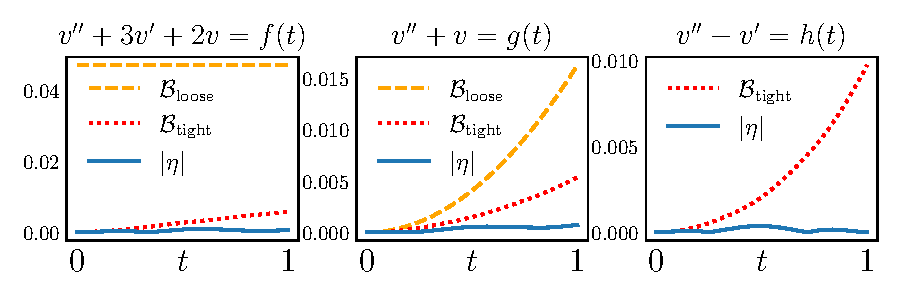
\includegraphics[width=\linewidth]{assets/2nd-order.pdf}
        \caption{\small
            Loose bound (Alg. \ref{alg:single-linear-ode-constant-coeff-loose}) and tight bound (Alg. \ref{alg:single-linear-ode-constant-coeff-tight}) for 3 second-order linear ODE with constant coefficients.
            Notice that the loose bound cannot be applied to the third equation since it has characteristic roots with positive real part.
        }\label{fig:2nd-order-bound} 
    \end{figure}

\subsection{LINEAR ODE SYSTEM WITH CONSTANT COEFFICIENTS} \label{section:high-dimension}
    \begingroup 
        \setlength\arraycolsep{1pt}
        In this part, we train $6$ networks to solve a $6$-dimensional linear system of ODEs with constant coefficients, namely, $\frac{\mathrm{d}}{\mathrm{d}t}\vect{v} + A\vect{v} = \vect{f}$. 
        We pick $A = PJP^{-1}$ where {\small $J=\begin{pmatrix}J_1\\[-0.75ex]&J_2\\[-0.75ex]&&J_3\end{pmatrix}$} with {\small $J_1 = \begin{pmatrix} 4&1\\[-0.75ex]&4&1\\[-0.75ex]&&4\\[-0.5ex]\end{pmatrix}$, $J_2 = \begin{pmatrix} 3&1\\[-0.75ex]&3\\[-0.5ex]\end{pmatrix}$ }, $J_3=2$, and $P$ is a random orthogonal matrix.
    \endgroup

    We pick the initial conditions to be $\vect{v}(0) = P(0\, 0\, 1\, 0\, 1\, 1)^{T}$ and the forcing function to be $\vect{f}(t) = P(\cos t + 4 \sin t  + \ln(1+t),\, \frac{1}{1+t} + 4 \ln(1+t) + (t+1),\, 4t + 5,\, 2t + 3t^2 + e^t,\, 4 e^t,\, 2 \cos t - \sin t )^T$, so that the manufactured exact solution is $\vect{v}(t) = P ( \sin t,\, \ln(t + 1),\, t + 1,\, t^2,\, e^t,\, \cos t)^T$.

    After obtaining the residual information $\vect{r}(t)=\frac{\mathrm d}{\mathrm d t}\vect{u}(t) + A\vect{u}(t) - \vect{f}(t)$, we apply Alg. \ref{alg:system-bound} to obtain componentwise bound and norm bound of $\pmb{\Err} = \vect{u}-\vect{v}$. See Fig. \ref{fig:system-bound}. It is shown in Fig. \ref{fig:system-bound} that the bounds hold true over the domain.

    \begin{figure}[!htp]
        \centering
        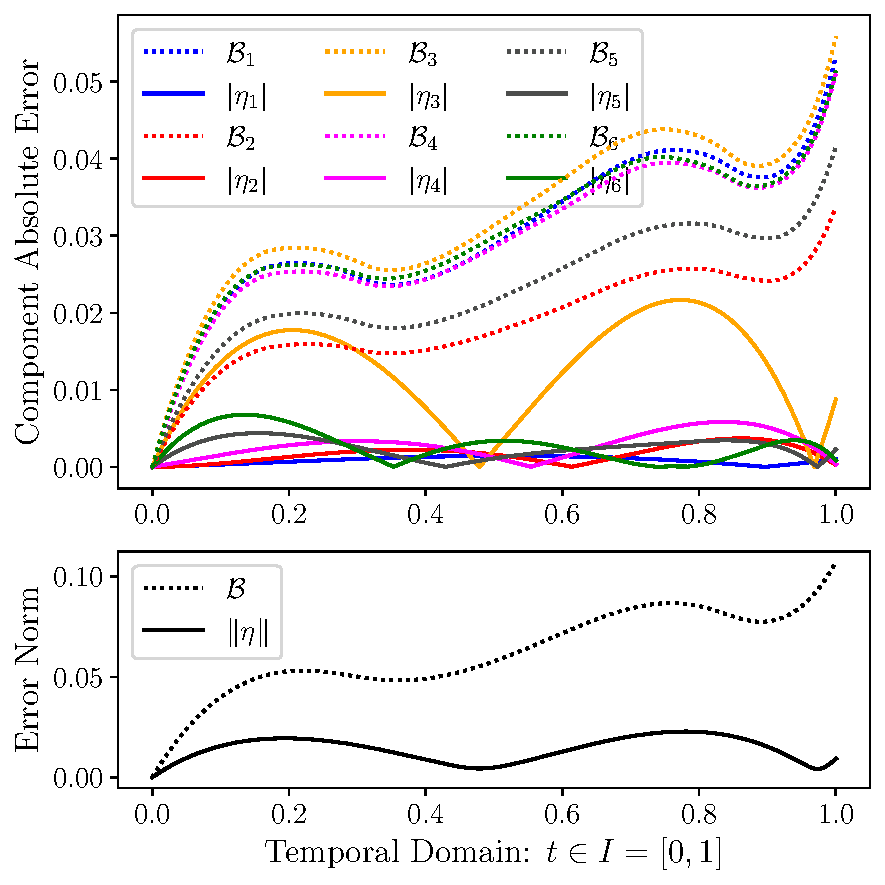
\includegraphics[width=\linewidth]{assets/system-bound.pdf}
        \caption{\small \textit{Componentwise} bound (upper) and \textit{norm} bound (lower) for linear ODE system with constant coefficients}\label{fig:system-bound}
    \end{figure}
% \subsection{LINEAR ODE SYSTEM WITH NONCONSTANT COEFFICIENTS -- NONHARMONIC OSCILLATOR} \label{section:experiment-nonharmonic-oscillator}
\subsection{NONLINEAR ODE -- DUFFING EQUATION} \label{section:experiment-duffing}
    In this part, we consider a Duffing oscillator, which is characterized by the following $2$nd order nonlinear ODE:
    \begin{equation}\label{eq:duffing}
        \frac{\mathrm{d}^2 v}{\mathrm{d}t^2} + 3 \frac{\mathrm{d}v}{\mathrm{d}t} + 2v +\varepsilon v^3 = \cos t ,
    \end{equation}
    under the initial conditions $v(0) = 1$ and $v'(0) = 1$, where $\varepsilon$ controls the nonlinearity of the equation. Using Alg. \ref{alg:nonlinear-iterative}, we solve the equation on $I=[0, 2]$ for linspaced $\varepsilon \in (-0.9, 0.9)$ using neural networks and bound the errors. The input $J$ to Alg. \ref{alg:nonlinear-iterative} is chosen to be $6$. Namely, we expand the solution and bound components from degree $0$ to $6$.

    The analytical solution to Eq. \ref{eq:duffing} is complicated. Hence, we use the RKF4(5) method to compute numerical solutions that are close enough to exact solutions for visualization purposes. See Fig. \ref{fig:duffing-solution} for network solutions compared against RKF4(5) and Fig. \ref{fig:duffing-error} for error bounds compared against true absolute error.
    \begin{figure}[!htp]
        \centering
        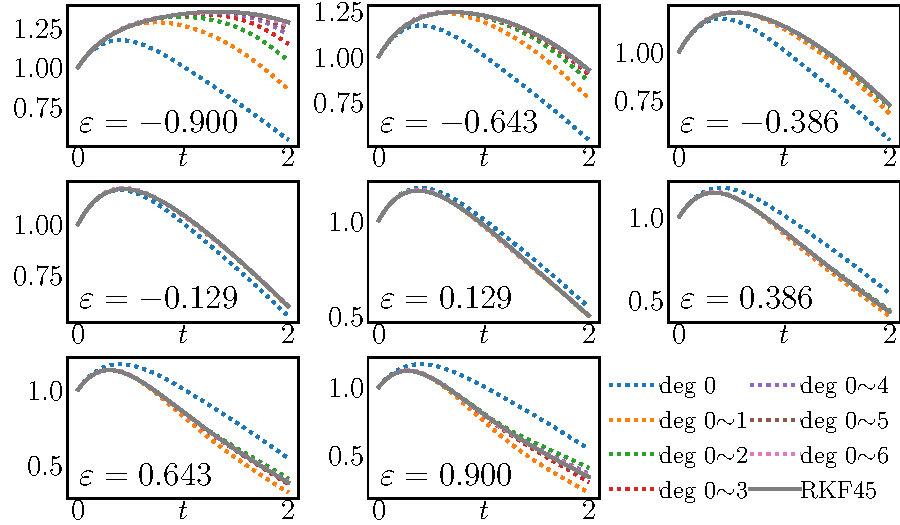
\includegraphics[width=\linewidth]{assets/duffing-solution.pdf}
        \caption{\small RKF45 and Network Solutions (max-degree 0$\sim$6) to Duffing equation \ref{eq:duffing} for $\varepsilon \in (-0.9, 0.9)$}\label{fig:duffing-solution}
        \vspace{1em}
        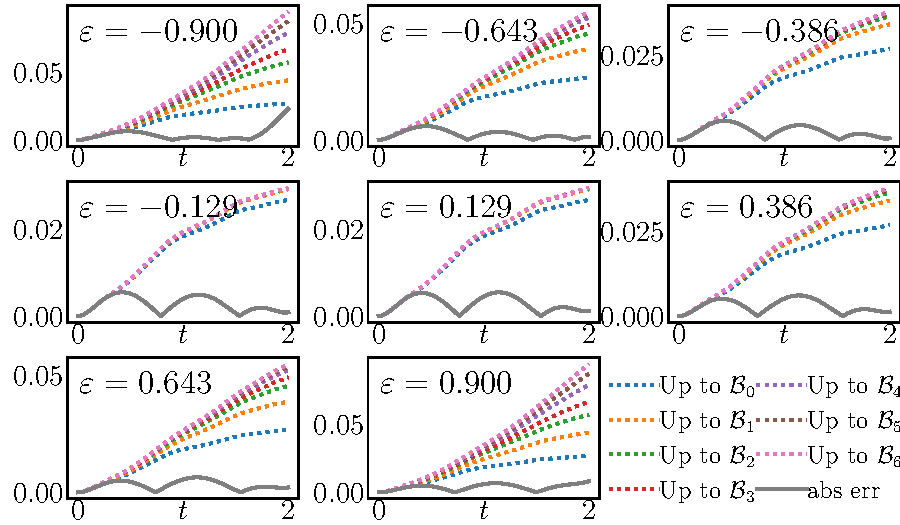
\includegraphics[width=\linewidth]{assets/duffing-error.pdf}
        \caption{\small True Error vs. error bound (max-degree 0$\sim$6) of neural network solution to Duffing Equation \ref{eq:duffing} for $\varepsilon \in (-0.9, 0.9)$}\label{fig:duffing-error}
    \end{figure}

\subsection{LINEAR PDE SYSTEM WITH NONCONSTANT COEFFICIENTS } \label{section:experiment-attractor}
    \begin{figure}[!htp]
        \centering
        \subfloat[\centering \small $\mathcal{C}: \begin{cases*} x' = -x - y \\ y' = x - y \end{cases*}$]{{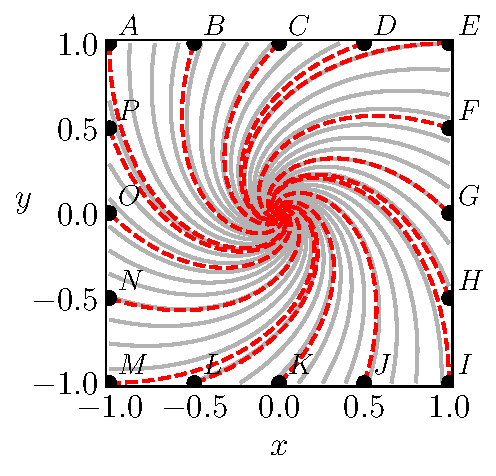
\includegraphics[width=0.50\linewidth]{assets/characteristics.pdf}}}
        \subfloat[\centering \small $\mathcal{C}: \begin{cases*} x' = x^2 + y^2 + 1 \\ y' = x^2 - y^2 + 2 \end{cases*}$]{{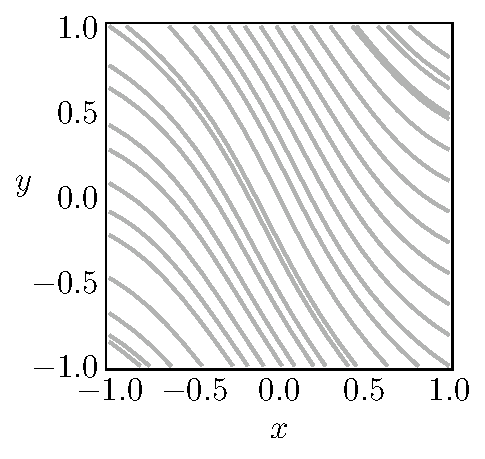
\includegraphics[width=0.49\linewidth]{assets/unsolvable-characteristics.pdf}}}
        \caption{
            \small
            Characteristics curves of Eq. \ref{eq:attractor} (left) and Eq. \ref{eq:hard-to-solve-characteristics} (right). 
            The red curves, with staring points $A$ to $P$, are selected for visualization of absolute error and error bound in Fig. \ref{fig:pde-error-bound}.
        }\label{fig:characteristics}
    \end{figure}

\subsubsection{PDE Error Bound Evaluation Using Alg. \ref{alg:linear-first-order-pde-general}}
    \begin{figure}[!htp]
        \centering
        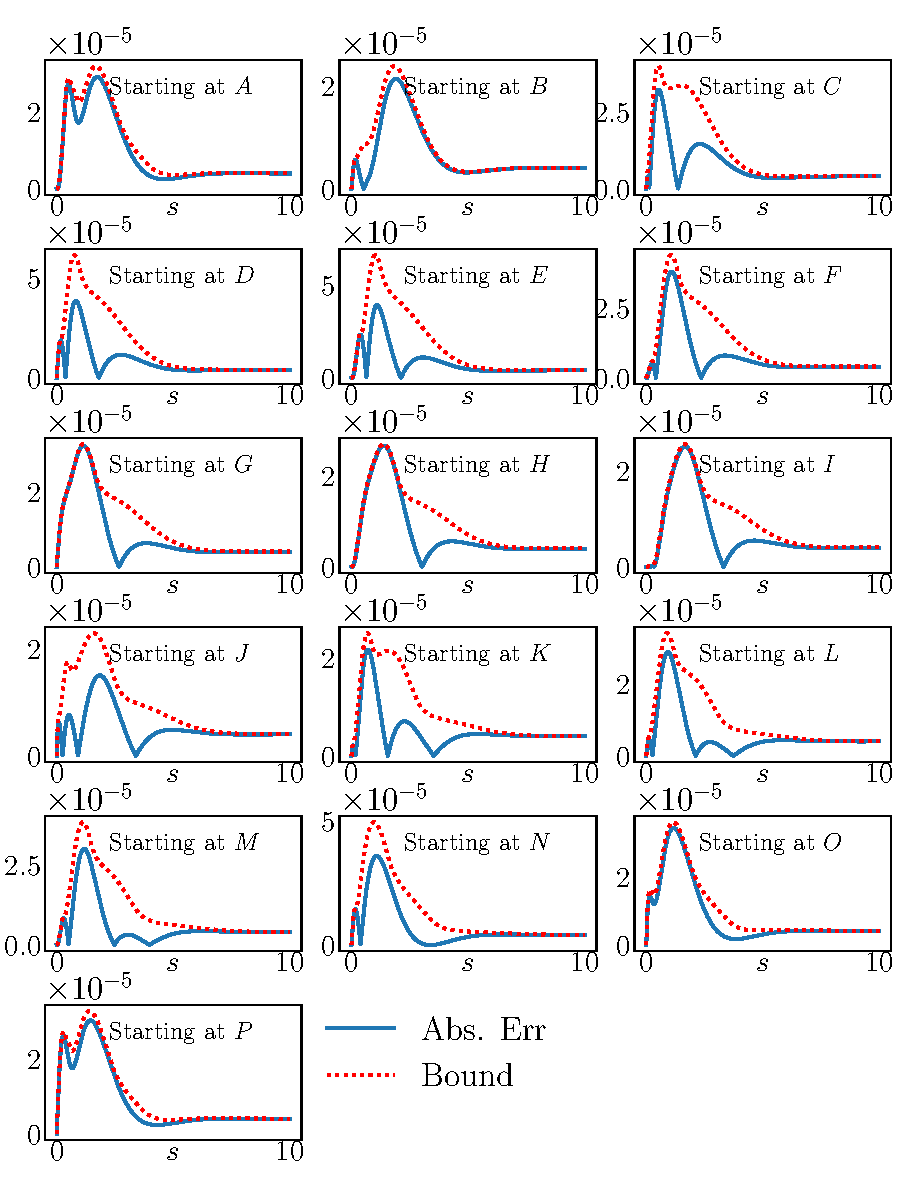
\includegraphics[width=\linewidth]{assets/pde-error-bound.pdf}
        \caption{
            \small
            Absolute error and error bound on selected characteristic curves. 
            These characteristic curve start at points $A$ through $P$ as shown in Fig. \ref{fig:characteristics}a.
            The blue solid curves are absolute error along the characteristic curves and red dotted curves are corresponding bounds.
        }\label{fig:pde-error-bound}
        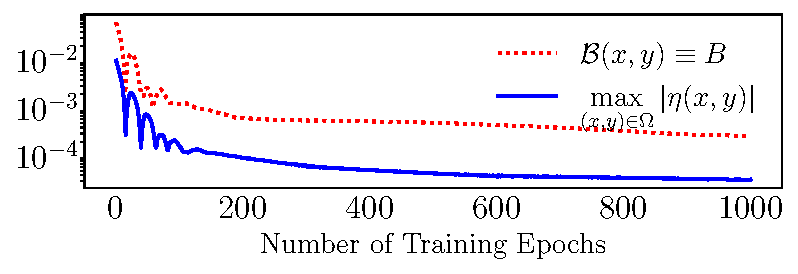
\includegraphics[width=\linewidth]{assets/pde-constant-bound.pdf}
        \caption{
            \small
            Constant bound $B$, computed using Alg. \ref{alg:linear-first-order-pde-constant}, and max absolute error over domain at different epochs of training.
        }\label{fig:pde-constant-bound}
    \end{figure}

    We try to solve the following first-order linear PDE,
    {
        \small
        \begin{equation} \label{eq:attractor}
            (-x -y) \partial_x v + (x - y) \partial_y v + v = 3x - 2y \text{ in } \Omega=[-1, 1]^2,
        \end{equation}
    }
    subject to the boundary constraints of $v(x, \pm1) =2x\pm 3$ and $v(\pm 1, y) = 3y \pm 2$. 
    The exact (manufactured) solution is given by $v(x, y) = 2x + 3y$.
    The characteristic curves are integral curves {\small $\mathcal{C}: \begin{cases*} x'(s) = -x - y \\[-0.25em] y'(s) = x - y \end{cases*}$}, which is sovled by {\small $\mathcal{C}: \begin{cases*} x(s) = R_0 e^{-s} \cos (s+\theta_0)\\[-0.25em] y(s) = R_0 e^{-s} \sin(s + \theta_0) \end{cases*}$}, where $R_0 = \sqrt{x_0^2+y_0^2}$ and $\theta_0 = \mathrm{atan2}(y_0, x_0)$ are constants determined by the starting point $(x_0, y_0) \in \Gamma = \partial \Omega$.
    See Figure \ref{fig:characteristics} for visualization.

    Since we know the analytical expression of the characteristic curves, we can apply Alg. \ref{alg:linear-first-order-pde-general} to estimate the bound on each characteristic curves. 
    We choose $16$ characteristic curves with starting points $A$, $B$, \dots, $P$, equidistantly placed on the boundary (Fig. \ref{fig:characteristics}a). 
    We plot the absolute error and the computed error bound along these characteristic curves in Fig. \ref{fig:pde-error-bound}.
    It can be seen that aboslute error lies strictly within the bounds.
\subsubsection{PDE Error Bound Evaluation Using Alg. \ref{alg:linear-first-order-pde-constant}}
    Consider the following PDE 
    {
        \small
        \begin{equation}\label{eq:hard-to-solve-characteristics}
            (x^2+y^2+1)\partial_x v + (x^2-y^2+2)\partial_y v + (3-2x)v = f
        \end{equation}
    }
    over domain $\Omega = [-1, 1]^2$, where $f(x, y) = 6-4x$.
    The boundary conditions are $v(-1, y) = v(x, 1) = 2$ and the manufactured solution is $v(x, y) = 2$.
    
    The characteristic curves {\small $\mathcal{C}: \begin{cases*} x'(s) = x^2+y^2+1 \\[-0.25em] y'(s) = x^2 - y^2 + 2 \end{cases*}$} are given by a nonlinear ODE, which are hard to solve analytically. 
    (See Fig. \ref{fig:characteristics}b for visualization)
    Therefore, Alg. \ref{alg:linear-first-order-pde-general} cannot be applied to evaluate the error bound. 

    However, the coefficient $(3-2x)$ is nonzero over domain $\Omega$.
    Hence, we can use Alg. \ref{alg:linear-first-order-pde-constant} to compute a constant error bound $|\eta(x, y)| \leq \Bound(x, y) \equiv B$ for all $(x, y) \in \Omega$.
    We visualize the bound and the maximum absolute error $\max_{(x, y)\in\Omega}|\Err|$ as a function of training epochs in Fig. \ref{fig:pde-constant-bound}.
    As expected, the bound is loose, which is about 1 order of magnitude larger than the max absolute error.
    Yet, it consistently holds true for every epoch, even during early stages of training, when the network performs poorly.
    % \begin{figure}[!htp]
    %     \centering
    %     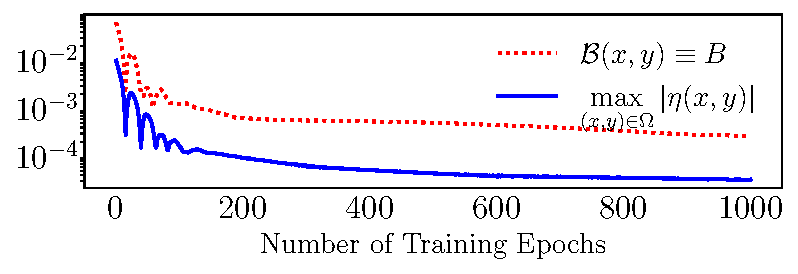
\includegraphics[width=\linewidth]{assets/pde-constant-bound.pdf}
    %     \caption{
    %         \small
    %         Constant bound $B$, computed using Alg. \ref{alg:linear-first-order-pde-constant}, and max absolute error over domain at different epochs of training.
    %     }\label{fig:pde-constant-bound}
    % \end{figure}

\section{Conclusion}
    In this paper, we propose various error bounding algorithms for PINN solutions to certain classes of ODEs and PDEs. 
    These algorithms only require the residual information $r(\cdot)$ and the equation structure $\mathcal{D} v = f$ as input.
    Using these algorithms, PINNs can be trained until error falls below specified tolerance.
    The mathematical relationship between residual and error bound also sheds light on optimizing PINN solutions for future studies.

\bibliography{references}


\end{document}
